\documentclass[tikz]{standalone}
\usepackage{pgfplots}
\pgfplotsset{compat=1.15}
\usepackage{mathrsfs}
\usetikzlibrary{arrows,calc}
\usepackage{tkz-euclide}
\pagestyle{empty}

\definecolor{AngleClr}{rgb}{0,0.39215686274509803,0}
\definecolor{ShapeClr}{rgb}{0.6,0.2,0}
\definecolor{SquareClr}{RGB}{250, 248, 217}

\begin{document}

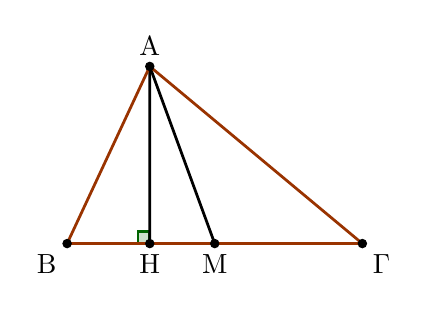
\begin{tikzpicture}[scale=.75]
\tkzSetUpLine[line width=1pt,color=black]
\tkzSetUpPoint[fill=black]

\tkzDefPoints{0/0/B,1.4/3/A,5/0/C}

\tkzDefMidPoint(B,C) \tkzGetPoint{M}
\tkzDefPointBy[projection=onto B--C](A)\tkzGetPoint{H}

\tkzFillPolygon[fill=white](A,B,C)

\tkzMarkRightAngle[line width=1pt, size=.2,color=AngleClr,fill=AngleClr,fill opacity=0.2](A,H,B)


\tkzDrawSegments[color=black](A,M A,H)
\tkzDrawPolygon[color=ShapeClr](A,B,C)

\tkzDrawPoints[size=3](A,B,C,M,H)

\tkzLabelPoint[above](A){$\rm A$}
\tkzLabelPoint[below](M){$\rm M$}
\tkzLabelPoint[below left](B){$\rm B$}
\tkzLabelPoint[below](H){$\rm H$}
\tkzLabelPoint[below right](C){$\rm \Gamma$}

\end{tikzpicture}

\end{document}
